\documentclass[11pt,a4paper]{article}

\usepackage[utf8]{inputenc}
\usepackage[T1]{fontenc}
\usepackage[spanish]{babel}
\usepackage[margin=2.2cm]{geometry}
\usepackage{graphicx}
\usepackage{hyperref}
\usepackage{booktabs}
\usepackage{enumitem}
\usepackage{xcolor}
\usepackage{titlesec}
\usepackage{fancyhdr}
\usepackage{float}

\hypersetup{colorlinks=true, urlcolor=blue, linkcolor=black}
\titlespacing*{\section}{0pt}{1.2ex}{0.6ex}
\titlespacing*{\subsection}{0pt}{0.9ex}{0.4ex}
\setlist{nosep}

\pagestyle{fancy}
\fancyhf{}
\fancyhead[L]{\small AlbaranIA --- Sprint 1}
\fancyhead[R]{\small Metodologías Ágiles}
\fancyfoot[C]{\thepage}

\title{\textbf{AlbaranIA} --- Informe Sprint 1 \\
\large Metodologías Ágiles $\cdot$ Universidad Europea}
\author{Lorena López Bermúdez \and Marcos García Manzano \and Camilo Andrés Sánchez Bernal}
\date{Abril--Mayo 2026}

\begin{document}
\maketitle

% ============================================================
\section{Contexto y objetivo}
% ============================================================

AlbaranIA es una plataforma SaaS multi-tenant para digitalizar albaranes
de proveedores mediante IA (GPT-4o Vision). Durante el Sprint~1 aplicamos
el marco Scrum documentando sus eventos (Planning, Dailies, Review,
Retrospectiva) y gestionando sus artefactos (Product Backlog, Sprint
Backlog, Incremento). El incremento comprometido cubría la base del
sistema: autenticación, gestión de usuarios y catálogo de proveedores.

El proyecto se gestiona en Jira (tablero ALB, board~133) y GitHub
(\texttt{albarania-scrum}). La coordinación del equipo se realizó
principalmente por Slack (\texttt{\#albarania-scrum}) y WhatsApp.

% ============================================================
\section{Equipo y roles}
% ============================================================

Los roles se acordaron el 24 de abril de 2026 por Slack y se registraron
en Jira al abrir el Sprint~1:

\begin{center}
\begin{tabular}{llp{7cm}}
\toprule
\textbf{Miembro} & \textbf{Rol Scrum} & \textbf{Responsabilidades principales} \\
\midrule
Lorena López Bermúdez & Scrum Master &
  Facilitación de eventos, gestión de impedimentos, criterios de aceptación, transparencia de artefactos \\
Marcos García Manzano & Product Owner + Developer &
  Priorización del backlog, redacción de historias de usuario, implementación técnica \\
Camilo A. Sánchez Bernal & Developer &
  Asignado a US-04 y US-06 (sin participación activa --- impedimento documentado) \\
\bottomrule
\end{tabular}
\end{center}

% ============================================================
\section{Product Backlog}
% ============================================================

El Product Backlog se organizó en 6~épicas, priorizadas por valor de negocio.
Para el Sprint~1 seleccionamos historias de E1 y E2:

\begin{itemize}
\item \textbf{E1 --- Autenticación y usuarios} (Alta): empresa, usuarios, login JWT, roles.
\item \textbf{E2 --- Catálogos} (Alta): CRUD y carga masiva de proveedores y artículos.
\item \textbf{E3 --- OCR} (Alta): subida de albaranes, extracción con IA, revisión.
\item \textbf{E4 --- Validación} (Media): máquina de estados, gate de ingeniería.
\item \textbf{E5 --- Facturación} (Media): agrupación, PDF, exportación ERP.
\item \textbf{E6 --- Dashboard} (Baja): métricas y reporting.
\end{itemize}

\noindent\textit{Nota: el Product Backlog fue creado y refinado por el
equipo AlbaranIA durante el Sprint~1, a partir de las épicas del proyecto
y el análisis del dominio. No se basó en un backlog predefinido externo.}

% ============================================================
\section{Sprint Planning}
% ============================================================

\subsection{Sprint Goal}

\begin{center}
\textit{``Construir la base: alta de empresa, usuarios, proveedores y login funcional.''}
\end{center}

\subsection{Historias seleccionadas (22~SP)}

\begin{center}
\begin{tabular}{lllcl}
\toprule
\textbf{Jira} & \textbf{ID} & \textbf{Historia} & \textbf{SP} & \textbf{Asignado} \\
\midrule
ALB-1 & US-01 & Crear empresa en la plataforma       & 5 & Lorena \\
ALB-2 & US-02 & Alta de usuarios con roles           & 3 & Lorena \\
ALB-3 & US-03 & Login con email y contraseña         & 3 & Marcos \\
ALB-4 & US-04 & Panel principal con navegación por rol & 3 & Camilo \\
ALB-5 & US-05 & CRUD de proveedores                  & 3 & Marcos \\
ALB-6 & US-06 & Importación de proveedores desde CSV & 5 & Camilo \\
\midrule
\multicolumn{3}{r}{\textbf{Total comprometido}} & \textbf{22} & \\
\bottomrule
\end{tabular}
\end{center}

Reparto inicial: Lorena 8~SP $\cdot$ Marcos 6~SP $\cdot$ Camilo 8~SP.
La asignación se acordó por autoorganización del equipo (Slack y WhatsApp,
15~abril) y se registró en Jira.

\subsection{Definition of Done}

\begin{itemize}
\item Código funcional (o mockup/prototipo representativo).
\item Revisado por al menos 1~compañero.
\item Documentado en el repositorio.
\end{itemize}

% ============================================================
\section{Ejecución del Sprint}
% ============================================================

\subsection{Daily Scrums}

Las dailies se realizaron por Slack (\texttt{\#albarania-scrum}) del 21
al 29 de abril. En la primera daily ya detectamos que Camilo no estaba
participando. Lo registramos como impedimento y aplicamos el ciclo de
gestión descrito en UA2-T01, sección~3.4.

\subsection{Impedimento crítico: ausencia de un miembro del equipo}

Camilo, asignado a US-04 y US-06 (8~SP), no participó en ninguna
actividad del sprint. Tras reiterados intentos de contacto y
ofrecimientos de participación por Slack y WhatsApp sin respuesta
sostenida, lo gestionamos siguiendo el ciclo de UA2-T01, sección~3.4:

\begin{enumerate}
\item \textbf{Detección:} desde la primera daily ($<$24~h).
\item \textbf{Clasificación:} organizacional, bloqueante, fuera del
  ámbito del equipo (Tabla~2, UA2-T01).
\item \textbf{Escalado:} comunicación al tutor, quien avaló documentar
  la ausencia como impedimento crítico.
\item \textbf{Resolución parcial:} nos reorganizamos con dos miembros
  activos. Marcos asumió la carga técnica; Lorena cubrió artefactos,
  criterios de aceptación y facilitación.
\item \textbf{Cierre y aprendizaje:} integrado en la Retrospectiva con
  acciones concretas para el Sprint~2.
\end{enumerate}

Decidimos no redistribuir forzosamente las historias de Camilo. Respetar
la autoorganización del equipo (UA2-T01, sección~4) implicaba no imponer
una solución desde arriba --- lo que la asignatura identifica como el
antipatrón de comando-control encubierto (UA2-T01, sección~3.6).

\subsection{Herramientas}

Jira (tablero ALB, board~133), GitHub (\texttt{albarania-scrum}),
Slack (\texttt{\#albarania-scrum}), WhatsApp. Convención de ramas
\texttt{feature/US-XX-*} y commits en español.

% ============================================================
\section{Sprint Review}
% ============================================================

\subsection{Incremento entregado}

\begin{center}
\begin{tabular}{llcl}
\toprule
\textbf{Historia} & \textbf{Descripción} & \textbf{SP} & \textbf{Estado} \\
\midrule
US-01 & Crear empresa en la plataforma & 5 & \textcolor{green!60!black}{Done} \\
US-02 & Alta de usuarios con roles & 3 & \textcolor{green!60!black}{Done} \\
US-03 & Login con email y contraseña & 3 & \textcolor{green!60!black}{Done} \\
US-05 & CRUD de proveedores & 3 & \textcolor{green!60!black}{Done} \\
\midrule
US-04 & Panel principal con navegación por rol & 3 & \textcolor{red!70!black}{Devuelta} \\
US-06 & Importación de proveedores desde CSV & 5 & \textcolor{red!70!black}{Devuelta} \\
\bottomrule
\end{tabular}
\end{center}

\textbf{Velocity: 14/22~SP = 64\,\%.} Las historias US-04 y US-06
volvieron al Product Backlog con comentarios formales en Jira
documentando el impedimento.

\subsection{Criterios de aceptación}

Redactamos 21 criterios en formato Given-When-Then para las 6~historias:
9 casos de éxito, 7 de error y 5 de validación de permisos. El Product
Owner los revisó y aprobó mediante Pull Request en GitHub (PR~\#1).

\subsection{Feedback recibido}

Incorporamos al backlog la historia \textbf{US-16: exportar proveedores
a CSV} y re-priorizamos \textbf{US-09 (OCR)} como historia ancla del
Sprint~2.

% ============================================================
\section{Retrospectiva}
% ============================================================

Aplicamos la técnica \emph{Start--Stop--Continue} (UA2-T02, sección~6):

\textbf{Start:}
\begin{itemize}
\item Definir criterios de aceptación Given-When-Then durante el Planning.
\item Política de reasignación si alguien falta a 2~dailies seguidas.
\end{itemize}

\textbf{Stop:}
\begin{itemize}
\item Asumir capacidad completa del equipo sin confirmar disponibilidad primero.
\end{itemize}

\textbf{Continue:}
\begin{itemize}
\item Dailies breves por Slack como canal principal de coordinación.
\item Tablero Jira como única fuente de verdad del estado del sprint.
\item Pair-review en Pull Requests.
\end{itemize}

\subsection{Acciones de mejora en Sprint~2}

\begin{itemize}
\item Capacidad ajustada a 13,5~SP (por debajo de la velocity) para
  dejar margen de seguridad.
\item Pareo SM$\leftrightarrow$PO en la arquitectura OCR, para mitigar
  el riesgo de bus factor.
\item Protocolo de reincorporación documentado para Camilo.
\end{itemize}

% ============================================================
\section{Evidencias del proceso en Jira}
% ============================================================

\subsection{Estado del sprint antes del cierre}

\begin{figure}[H]
\centering
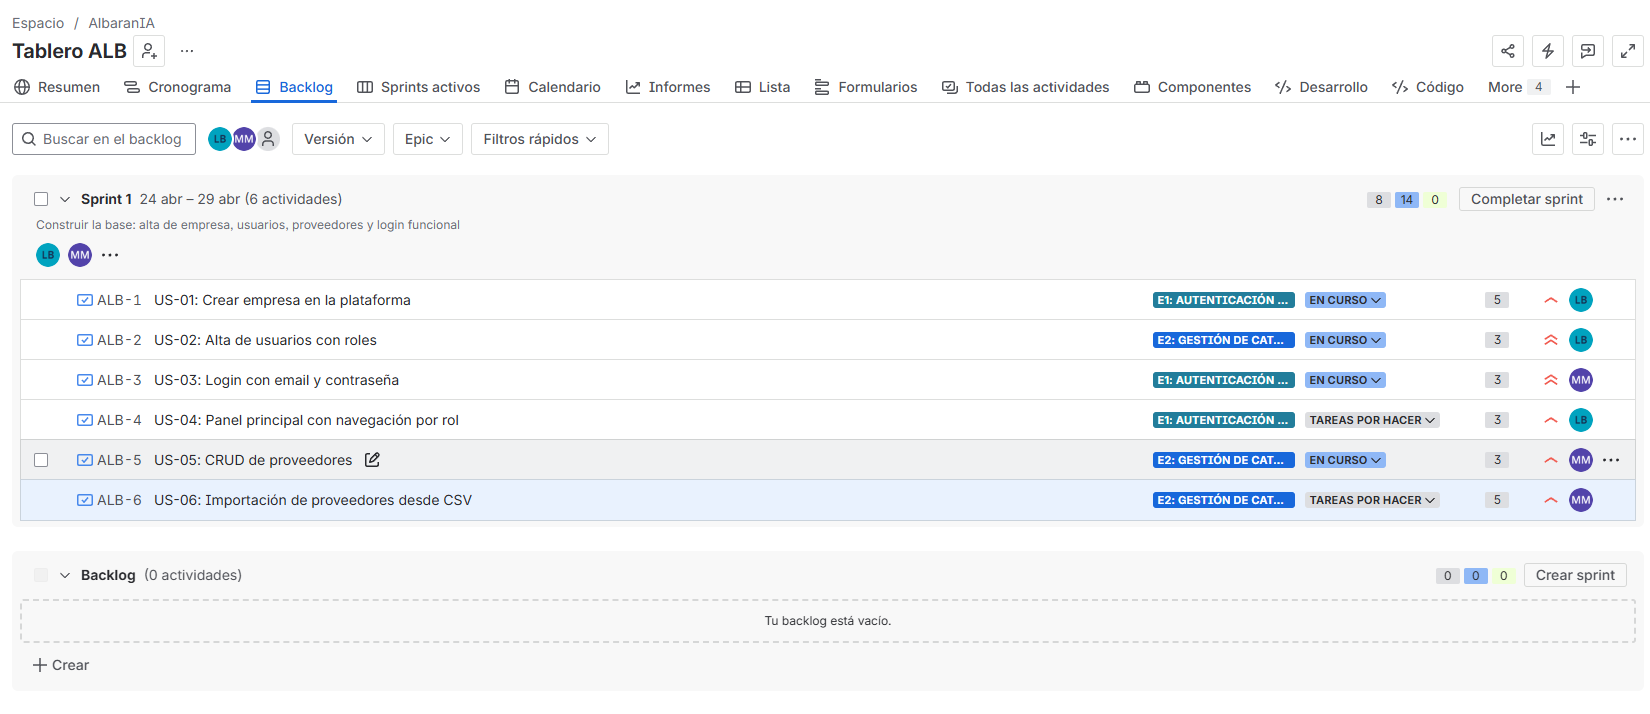
\includegraphics[width=0.48\textwidth]{01-backlog-pre-cierre.png}
\hfill
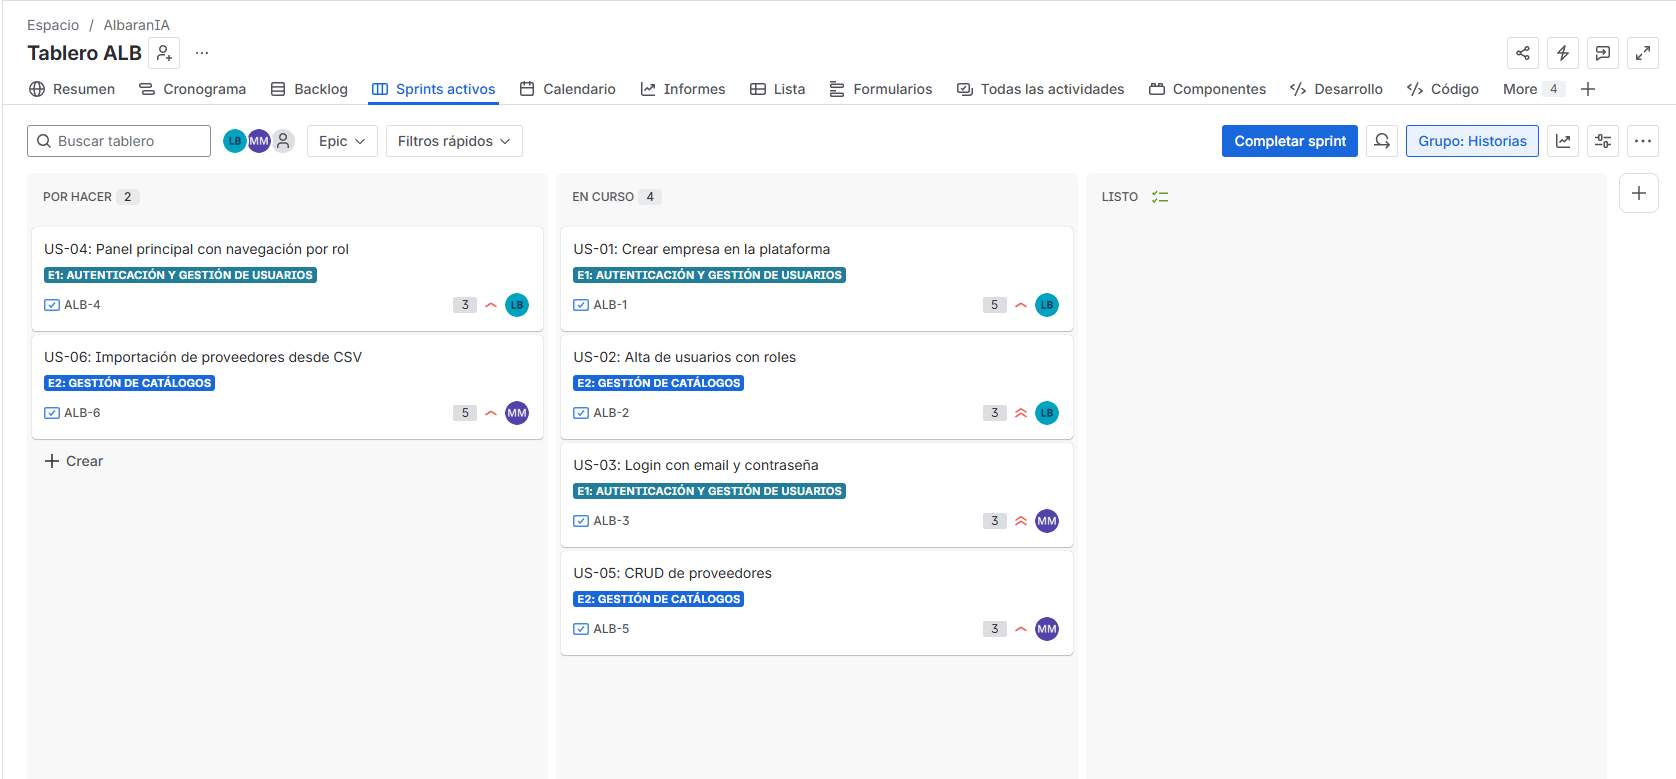
\includegraphics[width=0.48\textwidth]{02-tablero-board-sprint1.png}
\caption{(a)~Vista del backlog con las 6~historias del Sprint~1: 4 en
curso y 2 por hacer. (b)~Tablero Kanban mostrando el flujo de trabajo:
Por Hacer (ALB-4, ALB-6), En Curso (ALB-1, ALB-2, ALB-3, ALB-5),
Listo (vacío).}
\end{figure}

\begin{figure}[H]
\centering
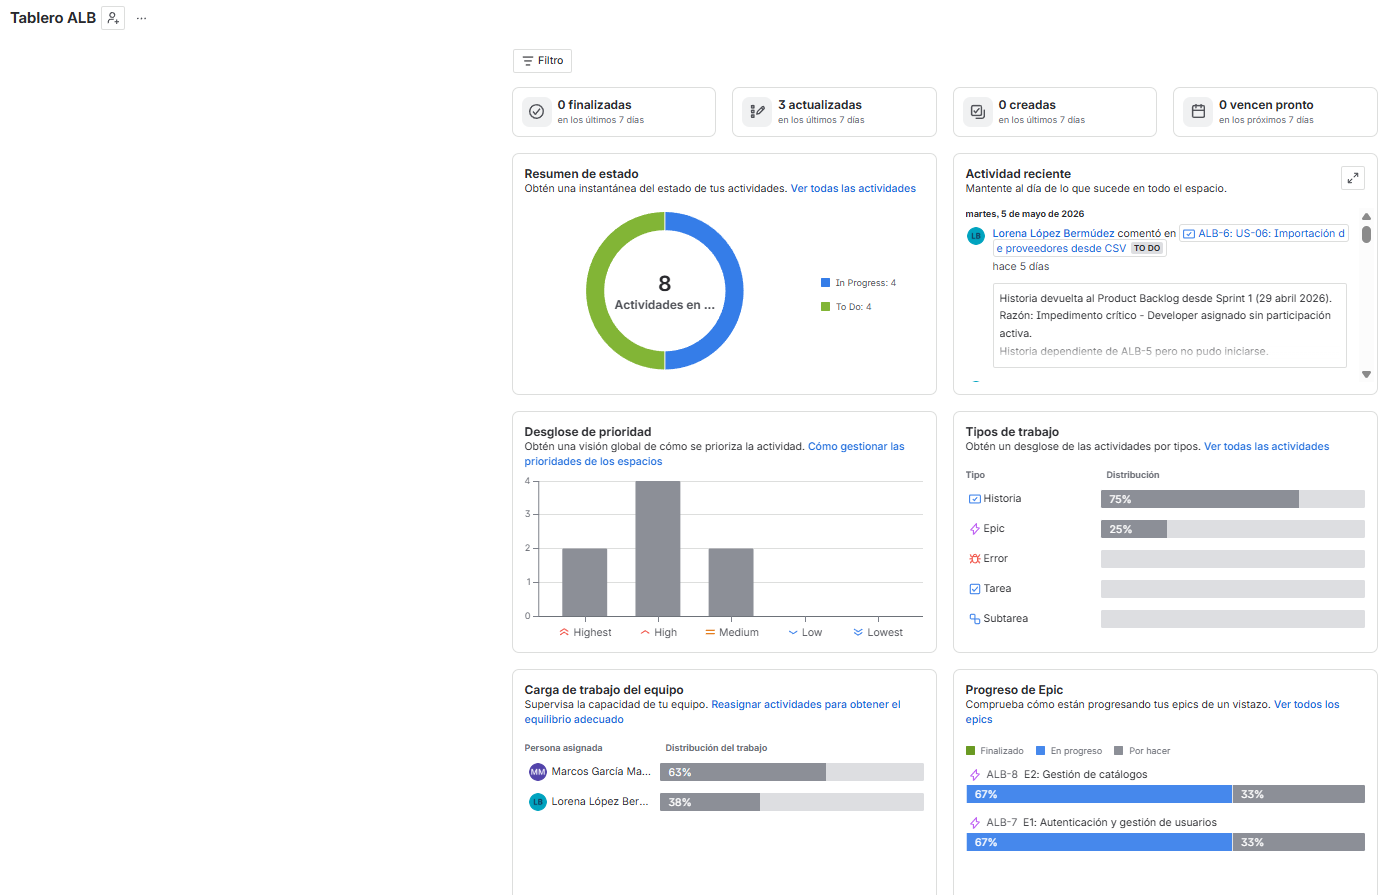
\includegraphics[width=0.7\textwidth]{03-resumen-metricas.png}
\caption{Panel de resumen: distribución de carga (Marcos 63\,\%,
Lorena 38\,\%), progreso de épicas E1 y E2 al 67\,\%, y actividad
reciente con los comentarios de devolución.}
\end{figure}

\subsection{Documentación del impedimento}

\begin{figure}[H]
\centering
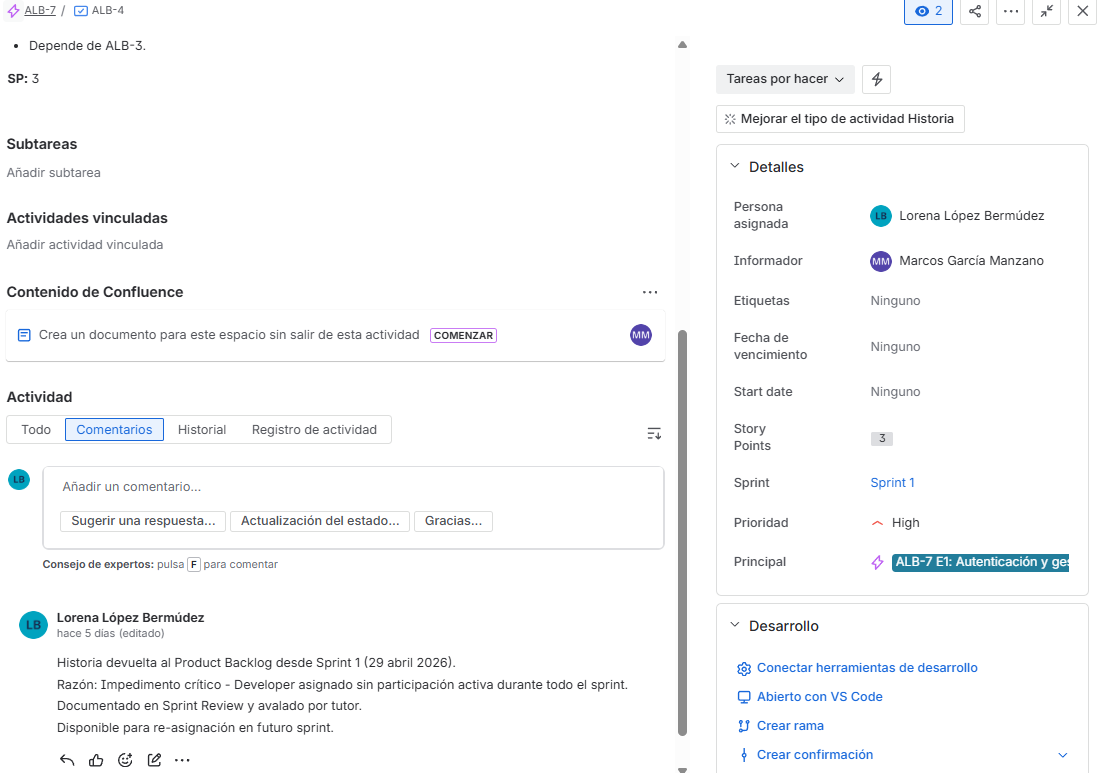
\includegraphics[width=0.48\textwidth]{04-comentario-devolucion-ALB4.png}
\hfill
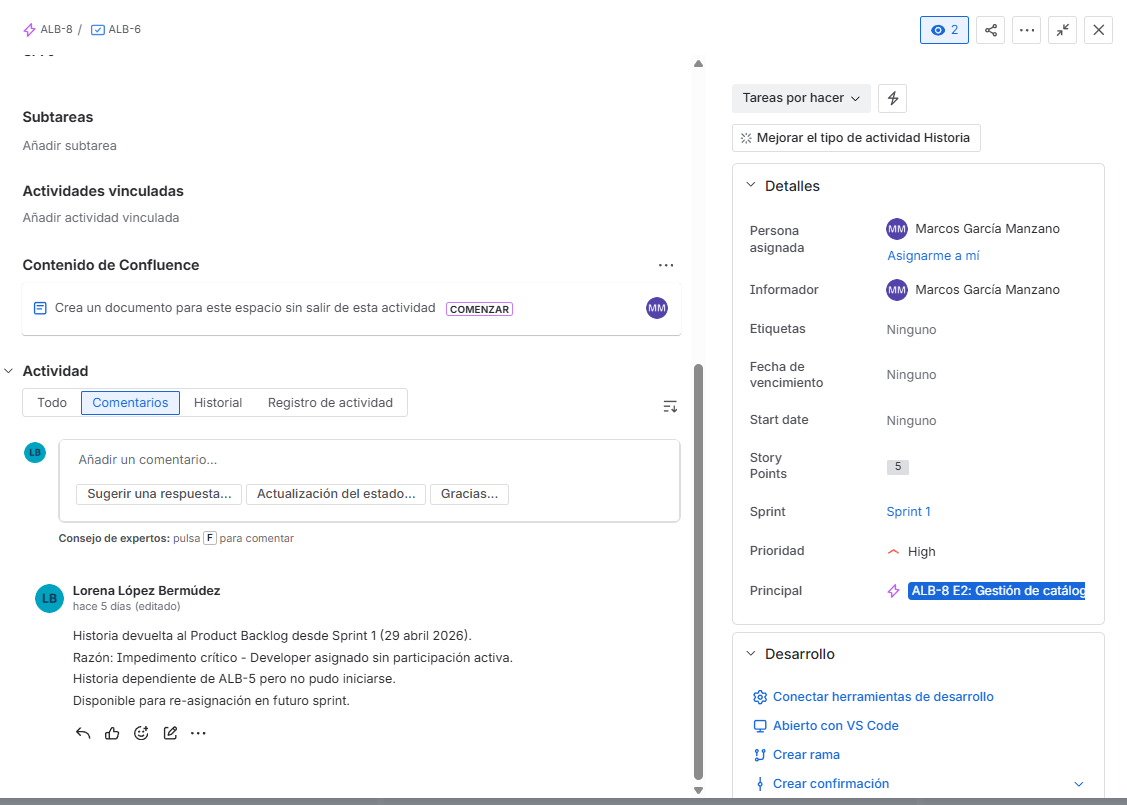
\includegraphics[width=0.48\textwidth]{05-comentario-devolucion-ALB6.png}
\caption{Comentarios formales de devolución al Product Backlog:
(a)~ALB-4 (US-04): impedimento crítico, avalado por tutor.
(b)~ALB-6 (US-06): impedimento crítico, historia dependiente de ALB-5.}
\end{figure}

\subsection{Proceso de cierre del Sprint~1}

\begin{figure}[H]
\centering
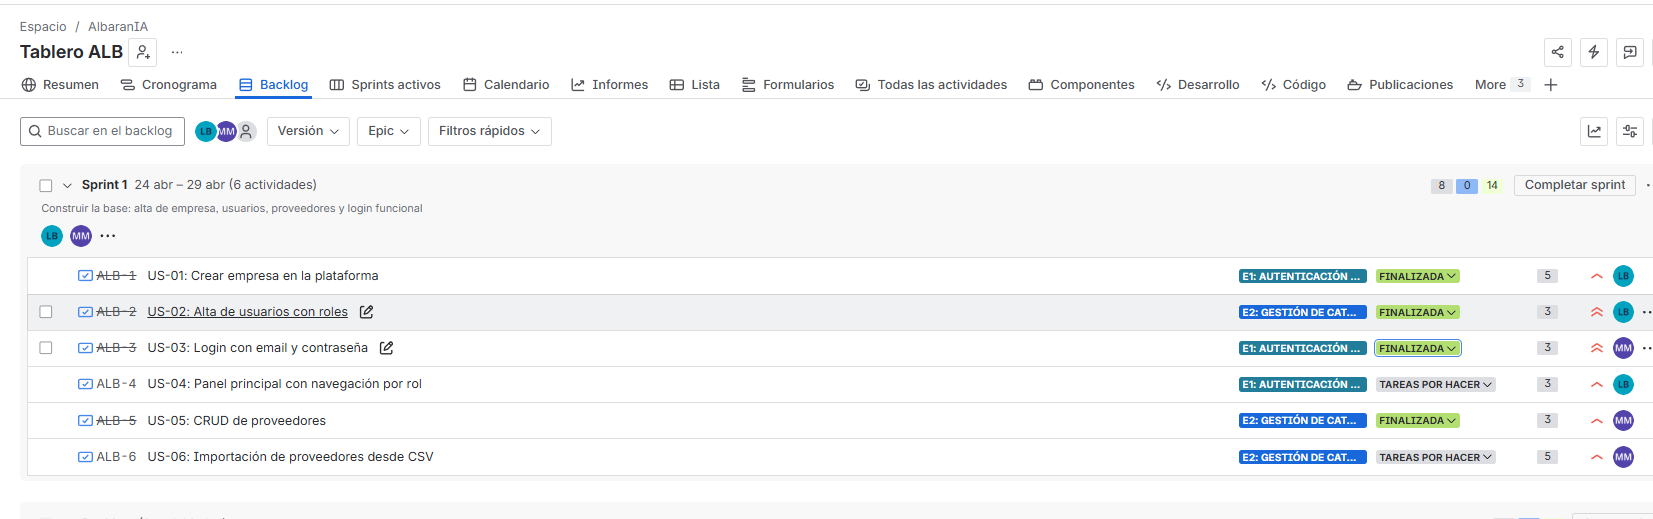
\includegraphics[width=0.45\textwidth]{06-backlog-4-finalizadas.png}
\hfill
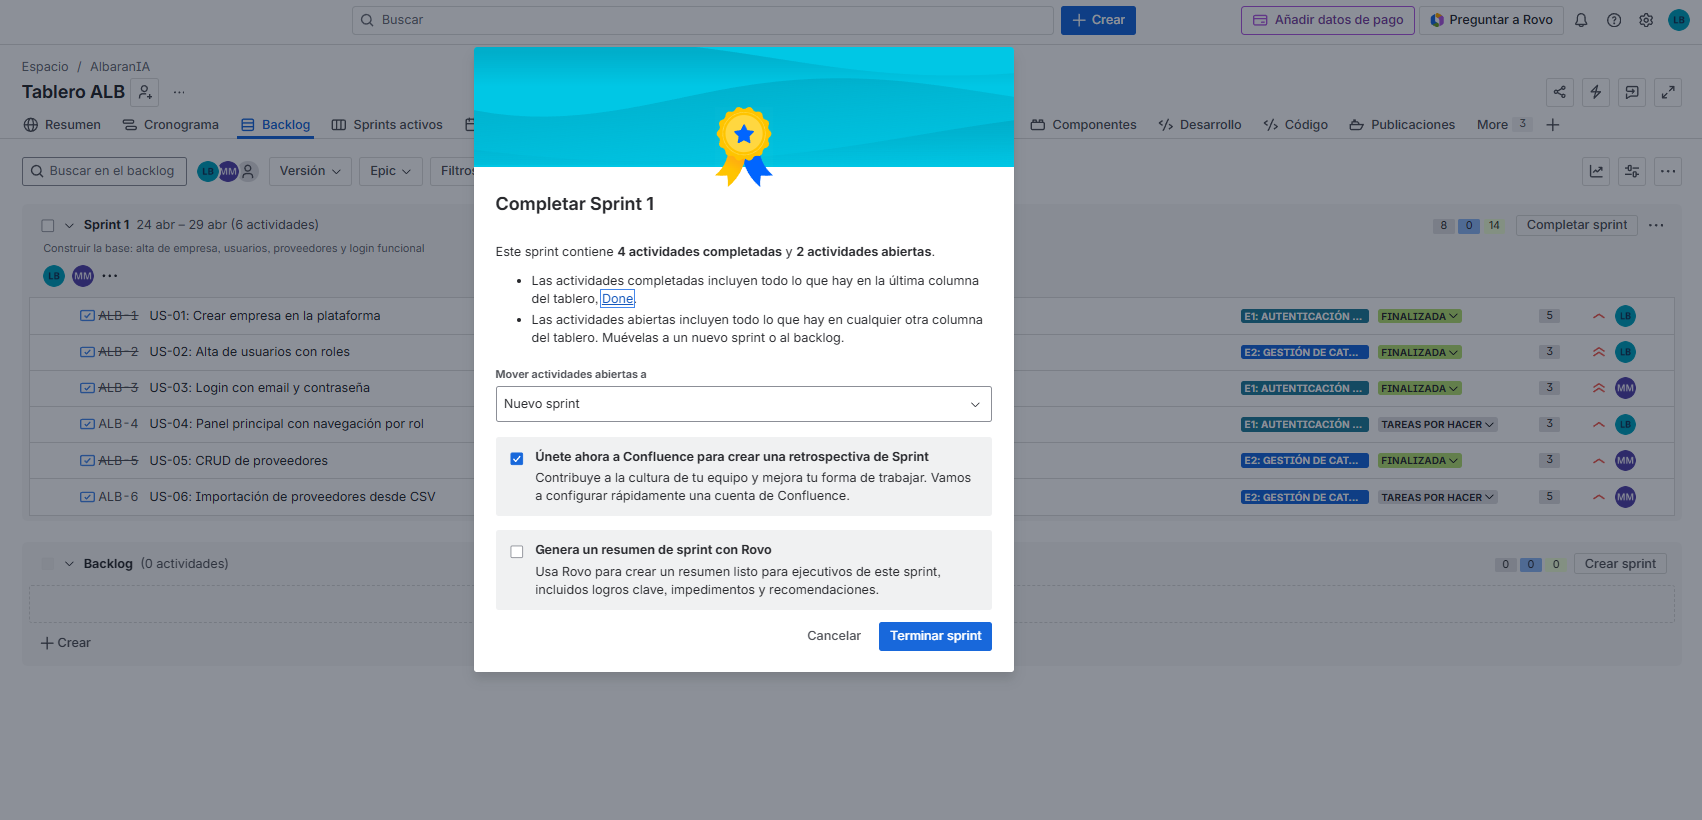
\includegraphics[width=0.45\textwidth]{07-dialogo-cierre-nuevo-sprint.png}

\vspace{0.3em}

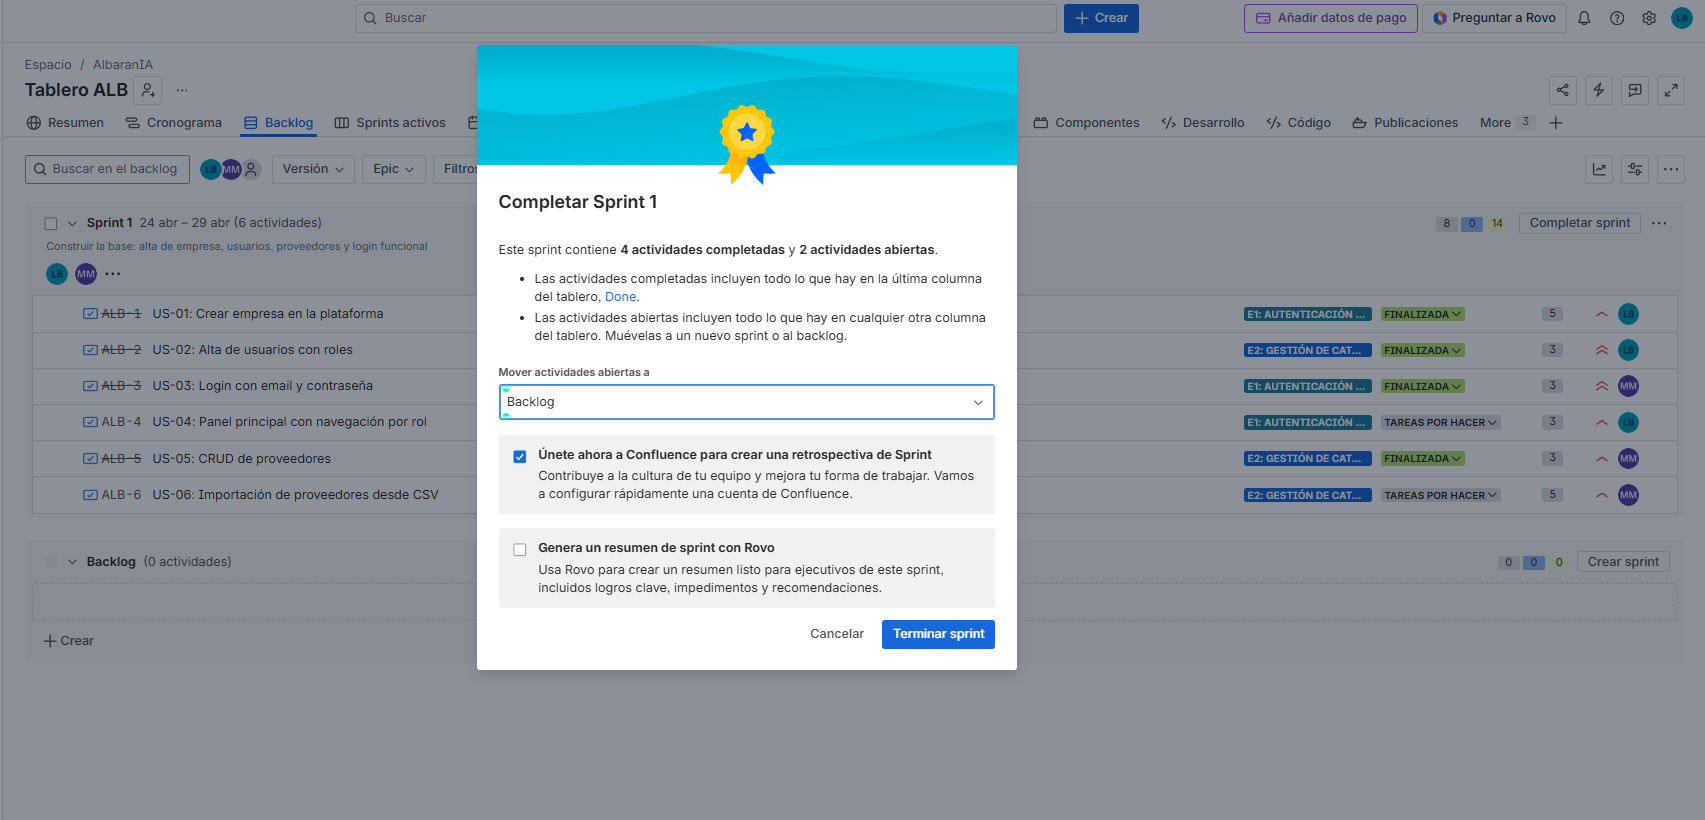
\includegraphics[width=0.45\textwidth]{08-dialogo-cierre-backlog.png}
\hfill
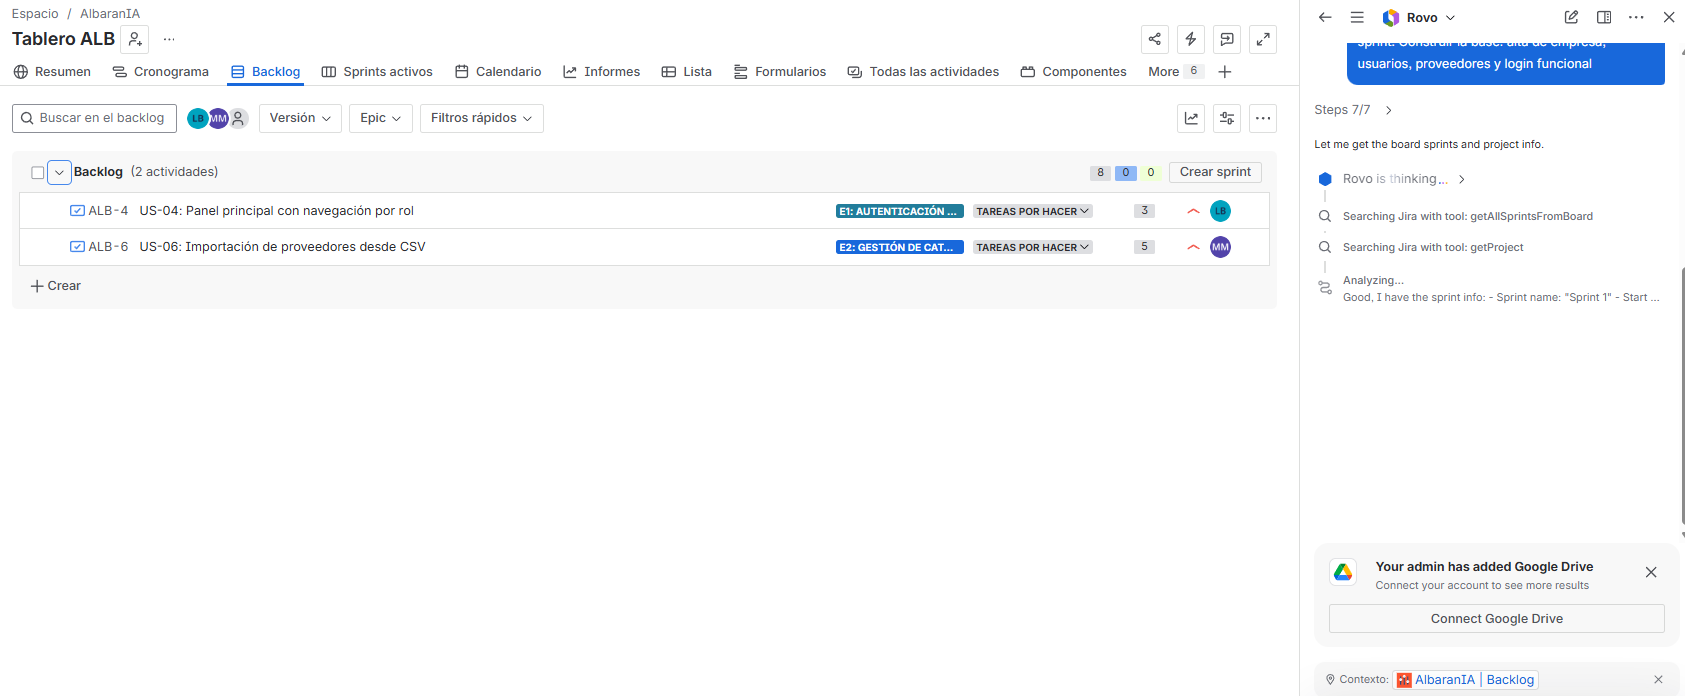
\includegraphics[width=0.45\textwidth]{09-backlog-post-cierre.png}
\caption{Secuencia de cierre: (a)~4 historias marcadas como Finalizada.
(b)~Diálogo de cierre inicial (opción ``Nuevo sprint'').
(c)~Selección de ``Backlog'' para devolver ALB-4 y ALB-6.
(d)~Resultado: backlog post-cierre con las 2 historias devueltas.}
\end{figure}

\subsection{Velocity del Sprint~1}

\begin{figure}[H]
\centering
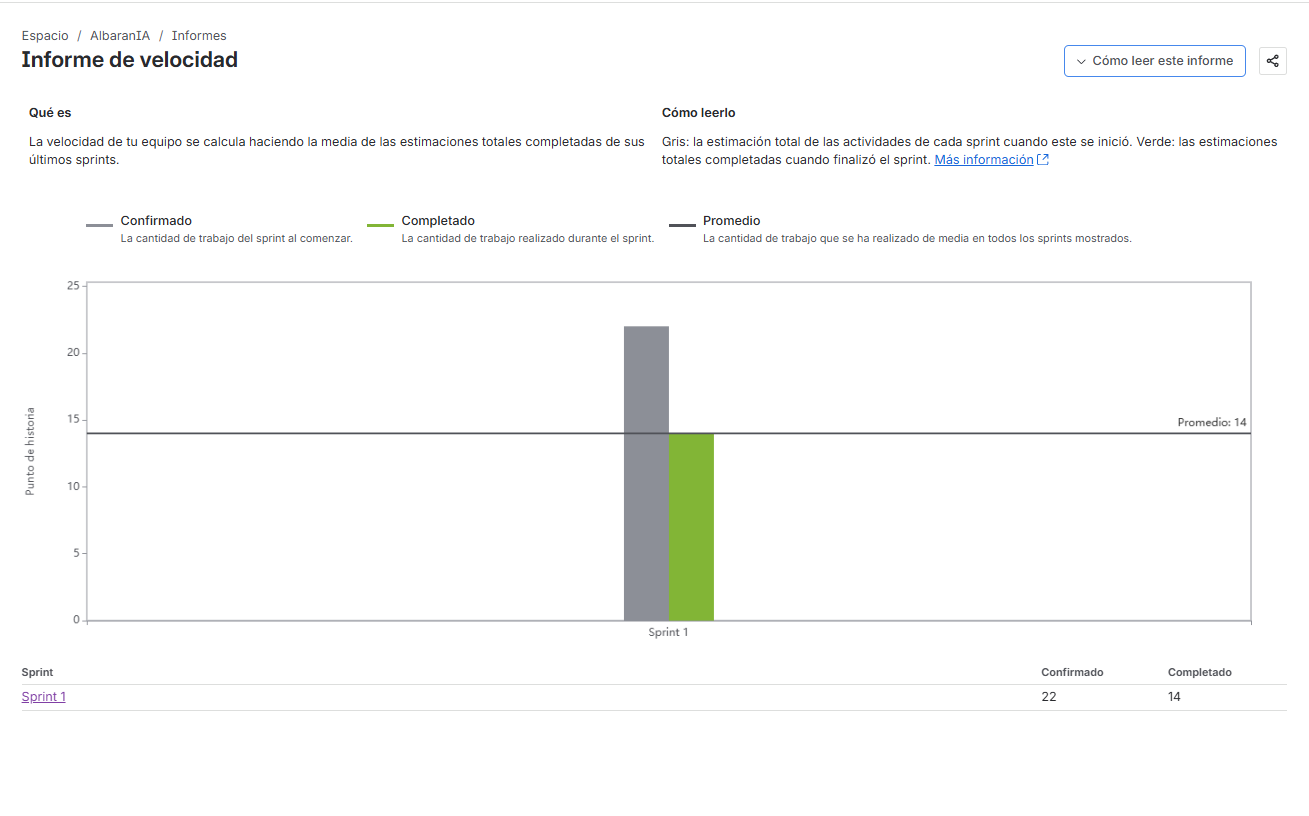
\includegraphics[width=0.7\textwidth]{10-velocity-chart.png}
\caption{Informe de velocidad generado por Jira: 22~SP comprometidos
(gris), 14~SP completados (verde). Velocity = 14~SP (64\,\%).}
\end{figure}

% ============================================================
\section{Conclusiones}
% ============================================================

El Sprint~1 cumplió parcialmente el Sprint Goal: entregamos 14~SP que
cubren autenticación, gestión de usuarios y catálogo de proveedores.
La velocity del 64\,\% no fue un fracaso --- fue información empírica.
Nos sirvió directamente para ajustar la capacidad del Sprint~2 a
13,5~SP con un equipo de dos miembros activos.

El impedimento de Camilo demostró que el ciclo de gestión funciona:
detectar, clasificar, escalar, resolver y aprender. Nos reorganizamos
sin necesidad de intervención directiva, respetando los roles del marco
Scrum.

Lo más importante que aprendimos: Scrum no garantiza que todo salga
según lo planificado. Lo que hace es darnos el marco para reaccionar.
Como recoge la Guía Scrum, el proceso empírico se apoya en
\textit{``inspección y adaptación continua''} \cite{scrumguide} ---
y eso es exactamente lo que hicimos. La mejora en el Sprint~2
(US-07 cerrada en Day~5, US-11 mergeada en Day~8) confirma que
el ciclo funcionó.

\vspace{1em}
\noindent\textbf{Enlaces:}
\begin{itemize}
\item Repositorio: \url{https://github.com/admin978/albarania-scrum}
\item Tablero Jira: \url{https://agente404.atlassian.net/jira/software/projects/ALB/boards/133}
\item PR criterios de aceptación: \url{https://github.com/admin978/albarania-scrum/pull/1}
\end{itemize}

% ============================================================
\begin{thebibliography}{9}
% ============================================================

\bibitem{scrumguide}
Schwaber, K., \& Sutherland, J. (2020). \textit{The Scrum Guide}.
\url{https://scrumguides.org/scrum-guide.html}

\bibitem{rubin}
Rubin, K.~S. (2012). \textit{Essential Scrum: A Practical Guide to the
Most Popular Agile Process}. Addison-Wesley.

\bibitem{cohn}
Cohn, M. (2025). \textit{Mountain Goat Software: Scrum and Agile}.
\url{https://www.mountaingoatsoftware.com/agile/scrum}

\bibitem{beck}
Beck, K., et al. (2001). \textit{Manifesto for Agile Software Development}.
\url{https://agilemanifesto.org}

\end{thebibliography}

\end{document}
